\newpage
\section{Scenario Editor}


\subsection{Introduction}
This chapter describes how to make use of the Scenario Editor (Figure \ref{ScenarioEditor}). When you open the editor, you see two main parts:
\begin{enumerate}
\item The Configuration panel, which is used to create, open and save configuration files.
\item The Entity panel, where a list of bots and a list of e-partners are being displayed. Here you can create, modify, rename and delete bots and e-partners.
\end{enumerate}

\begin{figure}[h]
\begin{center}
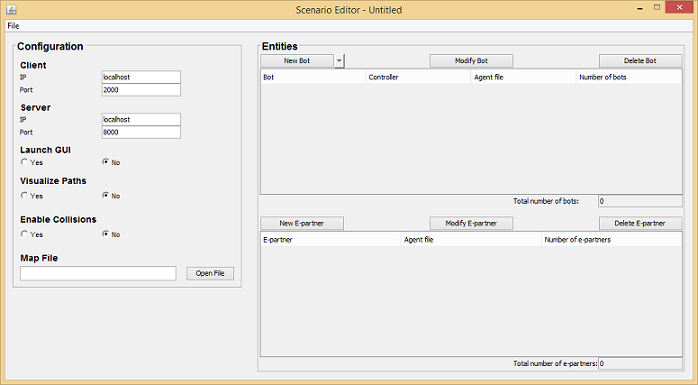
\includegraphics[width=0.9\textwidth]{ScenarioEditor/editor.png}
\caption{Scenario Editor}
\label{ScenarioEditor}
\end{center}
\end{figure}

\subsection{General use}
At the top of the editor you can see a $File$ menu. If you click on that, you get the options to create a new configuration, open an existing configuration, save your configuration, export your configuration and to exit the editor.

On the left side of the editor you can configure a scenario as you like. The Client IP, the Client Port, the Server IP and the Server Port should already contain the default values. You can change them if you need to. You can also indicate whether you want to open a GUI, visualise the paths the bots take or enable collisions. If you have a map file you want to use, you can import it by selecting the $Open$ $file$ button at the right section.

On the right side of the editor you can create, modify, rename and delete bots and e-partners. There also are a list of bots and a list of e-partners that are created, and below each list there is an indication of how many bots or e-partners are created in total.

Linked to the Scenario Editor are the Bot Store and the E-partner Store, which will also be discussed in this document.


\subsection{Configuration Panel}

% wrap figure does not play nice with item lists. But the alternative, having the pic just in the top
% of the page, is taking more space in the end.
\begin{wrapfigure}{r}{0.3\textwidth}
 \begin{center}
	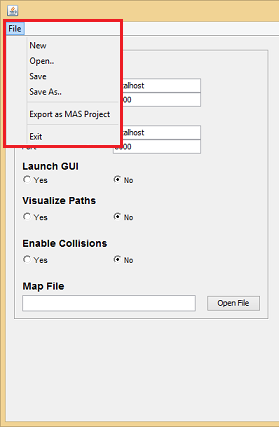
\includegraphics[width=0.3\textwidth]{ScenarioEditor/config.png}
 \end{center}
\caption{Configuration Panel}
\label{fig:ScenarioConfigPanel}
\end{wrapfigure}


A picture of the configuration panel can be found in Figure \ref{fig:ScenarioConfigPanel}. You have the following options:



\begin{itemize}

\item{New configuration file}:
To create a new configuration file, select $File$ $\to$ $New$ in the menu bar. You will now get a new configuration with the default values. Creating a new configuration will reset all previous changes you have made, so make sure you save your current configuration first if you want to keep it.


\item{Open configuration file}:
To open an existing configuration file, select $File$ $\to$ $Open$ in the menu bar. A window will pop up where you can select the folder where the configuration file is saved to. Once you have selected the right folder, select the file and click the $Open$ button.

\item{Save configuration file}:
To save your configuration file, select $File$ $\to$ $Save$ in the menu bar. If your file hasn't been saved before, a window will pop up where you can select the folder you want to save your configuration file to and enter the file name you want to use. Once you have selected the right folder and entered the file name, click the $Save$ button.

\item{Save configuration file as}:
To save your configuration in a new file, select $File$ $\to$ $Save$ $As$ in the menu bar. A window will pop up where you can select the folder you want to save your configuration file to and enter the file name you want to use. Once you have selected the right folder and entered the file name, click the $Save$ button.

\item{Export configuration to mas2g}:
To export your configuration to mas2g, you have to have saved your configuration first. Once you have done that, select $File$ $\to$ $Export$ $as$ $MAS$ $project$ in the menu bar. A window will pop up where you can select the folder you want to export the configuration to and the file name you want to use. Once you have selected the right folder and entered the file name, click the $Export$ $MAS$ $project$ button.

\emph{WARNING}: we recommend to use a relative file path to the configuration file. But currently, the generated mas2g file will contain an absolute path reference to the config file. We strongly recommend to fix the file reference in the mas2g file manually for cross-platform compatibility (so that others can also run your $MAS$).

\item{Exit the Scenario Editor}:
If you want to close the Scenario Editor, select $File$ $\to$ $Exit$ in the menu bar. Closing the Scenario Editor will not save any changes you have made, so make sure you save your configuration first if you want to keep it.
\end{itemize}



\subsection{Entity Panel}
The entity panel exists of 2 parts; the top part shows the bot options and the bottom part shows the e-partner options. A picture of the entity panel can be found in Figure \ref{fig:EntityPanel}. You have the following options:


\begin{figure}
\begin{center}
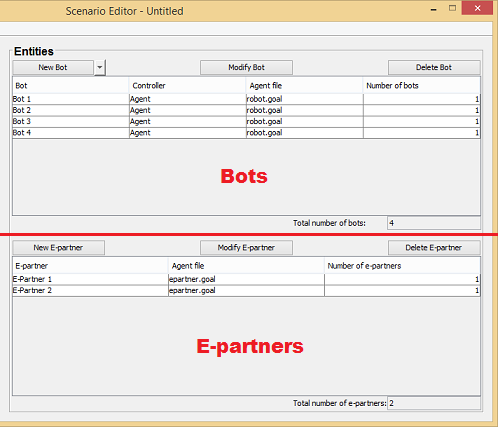
\includegraphics[width=0.6\textwidth]{ScenarioEditor/bot.png}
\end{center}
\caption{Entity Panel}
\label{fig:EntityPanel}
\end{figure}

\begin{itemize}
\item{Create new bot}:
To create a new bot, click the $New$ $Bot$ button. A new bot will appear in the bot list.\\
If you want to create a standard bot (which already has default values), click on the arrow next to the $New$ $Bot$ button. A menu will drop down where you can select one of the standard bots. If you click on one of the standard bots, the bot will appear in the bot list.

\item{Modify bot}:
To modify a bot, select the bot you want to modify in the bot list and click the $Modify$ $Bot$ button. The Bot Store will open in a new window where you can modify the properties of the bot.

\item{Rename bot}:
To rename a bot, you can either use the $Modify$ $Bot$ button to rename in the Bot Store, or you can rename in the Scenario Editor. To rename in the Scenario Editor, select the bot you want to rename in the list with bots. Double click the its name and enter a new name.

\item{Change controller type}:
To change how a bot is controlled, you can either use the $Modify$ $Bot$ button to change it in the Bot Store, or you can change it in the Scenario Editor. To change the controller type in the Scenario Editor, select the bot you want to change and click on its controller type. You should now be able to choose the controller type.

\item{Change the amount of entities of a bot}:
To change how many entities of a type of bot you want, you can either use the $Modify$ $Bot$ button to change it in the Bot Store, or you can change it in the Scenario Editor. To change the entity amount in the Scenario Editor, select the bot that you want to change the amount of. Now double click the amount given, and enter a new number.

\item{Delete bot}:
To delete a bot, select the bot you want to delete in the list with bots and click the $Delete$ $Bot$ button.

\item{Create new e-partner}:
To create a new e-partner, click the $New$ $E$-$partner$ button. A new e-partner will appear in the e-partner list.

\item{Modify e-partner}:
To modify an e-partner, select the e-partner you want to modify in the e-partner list and click the $Modify$ $E$-$partner$ button. The E-partner Store will open in a new window where you can modify the properties of the e-partner.

\item{Rename e-partner}:
To rename an e-partner, you can either use the $Modify$ $E-partner$ button to rename in the E-partner Store, or you can rename in the Scenario Editor. To rename in the Scenario Editor, select the e-partner you want to rename in the list with e-partners. Double click its name and enter a new name.

\item{Change the amount of entities of an e-partner}:
To change how many entities of a type of e-partner you want, you can either use the $Modify$ $E-partner$ button to change it in the E-partner Store, or you can change it in the Scenario Editor. To change the amount in the Scenario Editor, select the e-partner that you want to change the amount of. Now double click the amount given, and enter a new number.

\item{Delete e-partner}:
To delete an e-partner, select the e-partner you want to delete in the e-partner list and click the $Delete$ $E$-$partner$ button.

\end{itemize}


\subsection{Bot Store}
Figure \ref{fig:BotStore} shows a picture of the Bot Store. You have the following options:

\begin{figure}
\begin{center}
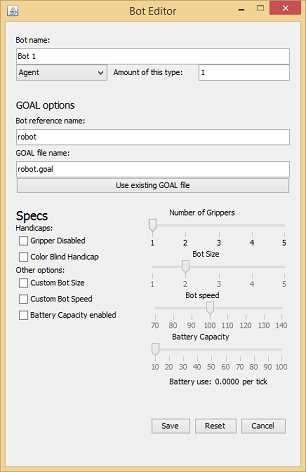
\includegraphics[width=0.4\textwidth]{ScenarioEditor/bs.png}
\end{center}
\caption{Bot Store}
\label{fig:BotStore}
\end{figure}

\begin{itemize}
\item{Rename bot}:
To rename a bot, click on the field that contains its current name. Now you are able to edit the current name or you can enter a new name.

\item{Change controller type}:
To change how a bot is controller, you can click on its current controller type. Now you are able to choose the controller type.

\item{Change the amount of entities}:
To change how many entities of the bot you want, you can click on the field that contains the current number of entities. Now you are able to edit the amount.

\item{GOAL options}:
You can enter the GOAL options for your bot under the $GOAL$ $options$ section. Here you can indicate what its reference name in GOAL should be, and you can select a GOAL agent file which will control the bot. To select the GOAL agent file, you can click on the $Use$ $existing$ $GOAL$ $file$ button. A window will pop up where you can select the folder where the GOAL file is saved to. Once you have selected the right folder, select the file and click the $Open$ button.

\item{Bot properties}:
You can find the available bot properties under the $Properties$ section. To change what properties you want the e-partner to have, you can select or deselect the checkbox next to the property description. Once you have enabled a property, you can use the sliders to change the value of that property.

\item{Save modifications}:
If you want to save the changes you have made to the bot, you can click on the $Save$ button. The Bot Store window will close, and your changes will have been saved.

\item{Reset modifications}:
If you want to reset the changes you have made to the bot, you can click on the $Reset$ button. Your changes will have been reverted to the last saved configuration.

\item{Cancel modifications}:
If you want to cancel modifying the bot without saving any changes, you can click on the $Cancel$ button. The Bot Store window will close.
\end{itemize}


\subsection{E-partner Store}
WARNING: The e-partner component of BW4T is not yet completely ready for use.

A picture of the E-partner Store is shown in Figure \ref{fig:epartnerstore}. You have the following options:

\begin{figure}[h]
\begin{center}
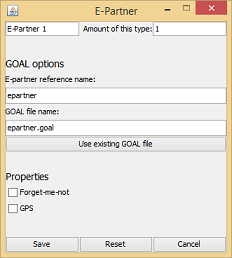
\includegraphics[width=0.4\textwidth]{ScenarioEditor/es.png}
\end{center}
\caption{E-partner Store}
\label{fig:epartnerstore}
\end{figure}

\begin{itemize}
\item{Rename e-partner}:
To rename an e-partner, click on the field that contains its current name. Now you are able to edit the current name or you can enter a new name.

\item{Change the amount of entities}:
To change how many entities of the e-partner you want, you can click on the field that contains the current number of entities. Now you are able to edit the amount.

\item{GOAL options}:
You can enter the GOAL options for your e-partner under the $GOAL$ $options$ section. Here you can indicate what its reference name in GOAL should be, and you can select a GOAL agent file which will control the e-partner. To select the GOAL agent file, you can click on the $Use$ $existing$ $GOAL$ $file$ button. A window will pop up where you can select the folder where the GOAL file is saved to. Once you have selected the right folder, select the file and click the $Open$ button.

\item{E-partner properties}:
You can find the available e-partner properties under the $Properties$ section. To change what properties you want the e-partner to have, you can select or deselect the checkbox next to the property description.

\item{Save modifications}:
If you want to save the changes you have made to the e-partner, you can click on the $Save$ button. The E-partner Store window will close, and your changes will have been saved.

\item{Reset modifications}:
If you want to reset the changes you have made to the e-partner, you can click on the $Reset$ button. Your changes will have been reverted to the last saved configuration.

\item{Cancel modifications}:
If you want to cancel modifying the e-partner without saving any changes, you can click on the $Cancel$ button. The E-partner Store window will close.

\end{itemize}